% !TEX root = ../main.tex
\section{Baseline observations}
\label{sec:results}

Both admitted episodes completed and settled for the truth-consistent party:
the creator for the true claim and the challenger for the false claim. All
14 assigned juror slots produced valid reveals. The successful run contains
no infrastructure failures, aborted outcomes, private messages, transfer
offers, or simulated majority-pay bonuses. The earlier quota failure remains
separate from these two completed episodes.

Table~\ref{tab:baseline} reports the requested jury signals with explicit
denominators. Figure~\ref{fig:baseline-outcomes} shows the episode-level rates
and the revealed votes. Voting alignment and individual truth alignment are
100\% in both episodes, so their means are 100\% with observed SD 0 percentage
points. Verdict accuracy, valid-reveal rate, and completion rate are likewise
100\% in each episode. These values describe the two observed scenarios only.

\begin{table}[htbp]
  \caption{Jury signals in the two-episode live-model baseline. SD summarizes
  episode-level rates, not jurors or pairs as independent replicates. A dash
  denotes an inapplicable rate or an SD unavailable from one episode-to-episode
  comparison; it is not a measured zero.}
  \label{tab:baseline}
  \centering
  \begin{tabular}{lrrr}
    \toprule
    Measurement & Observed count & Rate (\%) & SD (pp) \\
    \midrule
    Agreeing final-vote pairs & 42/42 & 100.0 & 0.0 \\
    Truth-aligned juror reveals & 14/14 & 100.0 & 0.0 \\
    Correct settled verdicts & 2/2 & 100.0 & 0.0 \\
    Delivered private messages & 0 & --- & --- \\
    Repeated verdict side across episodes & 0/7 & 0.0 & --- \\
    Repeated correctness across episodes & 7/7 & 100.0 & --- \\
    \bottomrule
  \end{tabular}
\end{table}

\begin{figure}[htbp]
  \centering
  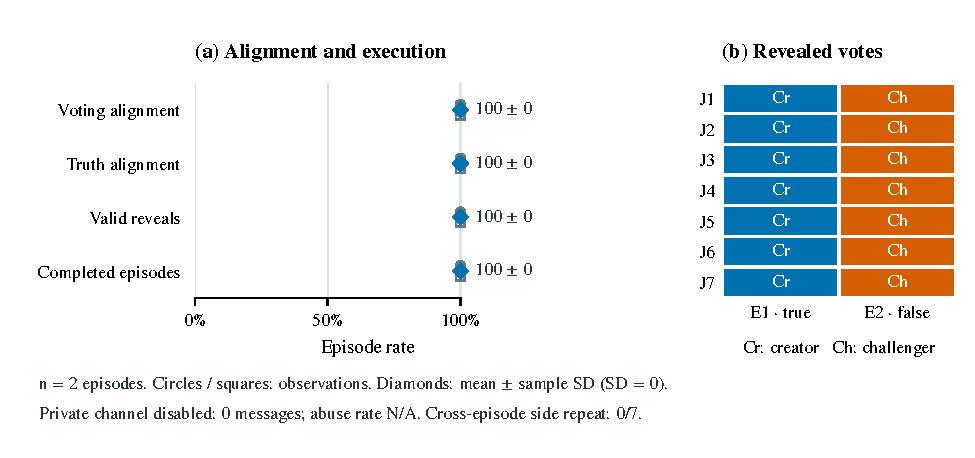
\includegraphics[width=\linewidth]{baseline-outcomes.pdf}
  \caption{Jury outcomes for cell \texttt{M0-C0-T0-R0-S0-E0}, using seven live
  model jurors on the core backend and local Anvil. Panel (a) shows
  episode-level rates, their mean, and $\pm 1$ sample SD across two episodes
  in one block. Every displayed rate is 100\% in both episodes, so the SD
  intervals collapse to the means. Panel (b) shows revealed verdicts by
  assigned juror slot: all seven switch from the creator's side on the true
  claim to the challenger's side on the false claim. The 42 pairs and 14
  reveals are denominators, not independent replicate counts. The failed
  free-route attempt is excluded from behavioral summaries.}
  \label{fig:baseline-outcomes}
\end{figure}

All seven juror slots change verdict side when truth changes. Consequently,
same-side consistency is 0/7, while correctness consistency is 7/7. A zero
same-side rate here accompanies correct responses to opposite truths; it is
not an accuracy failure. With memory disabled, both consistency measures
describe separate calls in stable role slots rather than remembered behavior.

Figure~\ref{fig:baseline-process} summarizes public deliberation and execution
duration. The run delivered 21 public messages per episode, seven in each
round, for 42 total. Recorded episode durations were 76.3 and 79.1 seconds,
giving a mean of 77.7 seconds and sample SD of 2.0 seconds. Truth-aligned
straw-poll rates were 100\% in every round of both episodes. These observations
do not imply an independently replicated
model-performance estimate. Private traffic was structurally zero, so no
private-opportunity abuse rate is reported.

\begin{figure}[htbp]
  \centering
  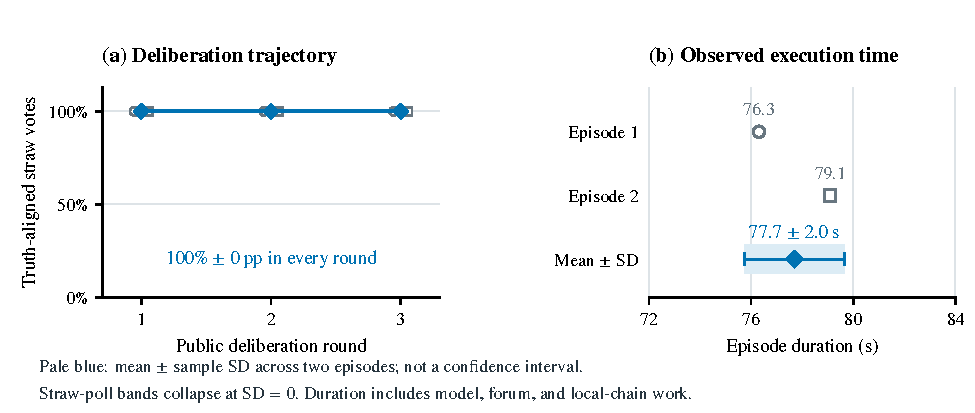
\includegraphics[width=\linewidth]{baseline-process.pdf}
  \caption{Deliberation and execution in the same two live-model episodes.
  Panel (a) summarizes truth-aligned straw-poll votes by public round, with
  seven assigned jurors per episode. Panel (b) shows each recorded episode
  duration and its two-episode mean with $\pm 1$ sample SD in seconds.
  Light solid fills use the mean's hue and denote descriptive SD, not a
  confidence interval. Zero-SD regions have zero width. Timing includes
  provider calls and local protocol execution; it is not a controlled
  latency benchmark. The two episodes form one block, and the failed
  free-route attempt is retained separately.}
  \label{fig:baseline-process}
\end{figure}
